\documentclass[runningheads,a4paper]{llncs}
\usepackage[left=3.0cm,right=3.0cm,top=2.5cm,bottom=4.5cm]{geometry}

\usepackage{url}
\usepackage{xparse}
\usepackage{amssymb}
\usepackage{graphicx}
\setcounter{tocdepth}{3}
\usepackage[linesnumbered,ruled,noline]{algorithm2e}

\newtheorem{thm}{Theorem}
\newtheorem{defn}{Definition}
\newtheorem{hyp}{Hypothesis} 
\newtheorem{exm}{Example} 

\NewDocumentCommand{\ceil}{s O{} m}{%
  \IfBooleanTF{#1} % starred
    {\left\lceil#3\right\rceil} % \ceil*[..]{..}
    {#2\lceil#3#2\rceil} % \ceil[..]{..}
}  

\newcommand{\keywords}[1]{\par\addvspace\baselineskip
\noindent\keywordname\enspace\ignorespaces#1}

\begin{document}
\mainmatter  

\title{Improved Cryptanalytic of Time-memory Trade-off Based on Rainbow Table}

\titlerunning{Improved Cryptanalytic of Time-memory Trade-off Based on Rainbow Table}

\author{Yulong Tian\textsuperscript{1} \and Dawu Gu\textsuperscript{1} \and Haihua Gu\textsuperscript{1,2}\and Ning Ding\textsuperscript{1}}
\institute{\textsuperscript{1,2}Computer Science and Engineering Department\\
Shanghai Jiao Tong University\\
200240 Shanghai,P.R. China\\
\textsuperscript{2}Shanghai Huahong Integrated Circuit Co.,Ltd\\
201203 Shanghai,P.R. China\\
\email{mathewes@sjtu.edu.cn, dwgu@sjtu.edu.cn\\
guhaihua@shhic.com, dingning@sjtu.edu.cn}\\
}

\maketitle


\begin{abstract}
Cryptanalytic time-memory trade-off (TMTO) has been studied for thirty years since the original paper of Hellman and has benefited from several important variants. Rainbow Table is one of the best known methods among all variants of TMTO. many improvments have been recommended since the Rainbow Table was proposed. However, most researchers concerned about either the time or the space, while little attention was paid to both the time and the space at the same time. In our work, we find out a new method to measure performance for both the time and the memory and all of our discussion are measured by the criteria. Under this method, we give out two optimization techniques based on the Rainbow Table. The first method is derived from the parameter selection and the best parameters. This method can reduce the cryptanalysis time by $28\%$ or the memory by $15\%$ compared with previous work. The second improvement is derived from the benefit of classic table. We present an improved table structure and it can benefit from the Rainbow Table and the Classic TMTO Table at the same time. Improved Table Structure can reduce the cryptanalysis time by $25\%$ with the cost of $5\%$ in success rate. In the rest of this paper, we combine two methods together and we show the final improvments with experiments. We also show that our methods can be further optimized under different conditions. As an example, we have implemented an attack platform for MS-Windows password hashes and all experiments are performed on this platform. 
\keywords{Time-Memory Trade-Off, Rainbow Table, Metric Scale, Improved Table Structure, NTLM}
\end{abstract}


\section{Introduction}

Brute-force and Look-up table \cite{borst1998time} could be used to solve most of hash-based \cite{rogaway2004cryptographic} cryptanalytic problems. However, in practice, these methods both have obvious limitation. The previous one will  will spend too much time and the later one will require unacceptable space. Thus, time-memory trade-off (TMTO) proposed by Hellman in 1980s \cite{hellman1980cryptanalytic} is a worthy replacement. The fundamental idea of TMTO is to carry out an exhaustive search only once and all following instances of the original problem become easy to solve.

\subsection{Previous works}

In 1980 \cite{hellman1980cryptanalytic}, Hellman presented the TMTO and gave out a choice for parameters which satisfied $m = t^2$. He suggested a method that can recover a key with $N^{\frac{2}{3}}$ unit of time and $N^{\frac{2}{3}}$ unit of memory. Cycle and Merge \cite{quisquater1990easy} shown in \textbf{Figure 1} are two flaws of classic tables. Cycle happens when two point are same to each other and merge happens when two points in the same columns are same to each other. With the increase of table, the probability of cycle and merge will increase significantly. Therefore, one of leakages in Hellman's paper is that the size of the single table should be limited. To avoid this problem, Rivest and Oechslin introduced different variants of TMTO. 

\begin{figure}
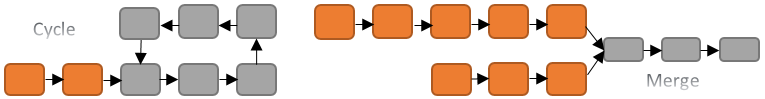
\includegraphics[width=\linewidth]{graph1}
\caption{Cycle and Merge. Cycle happens when same point in the chain is detected. Merge happens when two points in same column are same to each other. Cycle and merge will seriously afffect the performance of single table. Thus, the table size should be limited. }
\label{Figure 1}
\end{figure}

In 1982 \cite{rivest1978method} \cite{standaert2003time}, Rivest used the Distinguish Points, which has speical property such as ending up with ten zero , to detect cycyle and merge. Therefore, it can be used to construct large table. However, the Distinguish Point suffers cons from the variable length as it will increase the number of chains needed. So, the overhead of is far more large than the Hellman's Table in the number of chains.

No new optimisations have been published ever since then. In 2003 \cite{oechslin2003making}, Oechslin introduced the a revolutionary change of trade-off based on rainbow table and used it to demonstrate the efficiency by  recovering the passwords of Windows XP. In rainbow table, the reduction functions in different columns are different. Therefore, two different chains can merge if and only if at least two values in the same columns are same. The different reduction functions won't invoke the cycle at the same time. Thus, it can be used to generate large tables. Oechslin suggested that his method can reduce by two the number of calculations needed during cryptanalysis compared with the Hellman's Table. 

In 2006 \cite{barkan2006rigorous}, Barkan described a general model of TMTO and gave out the rigorous bound of different variants. They stated that almost all variants are the same. In the rest of their work, they proposed several new variants of time-memory-data trade-off and these variants takes advantage of both the the Hellman's Table and the Rainbow Table. Therefore, in our paper, we try to combine all variants together and take advantage of all variants of TMTO.

Therefore, this paper focuses on the optimization of the rainbow table and We will also discuss some of the advantages of the traditional method of TMTO.

\subsection{Existing Problems}

After Rainbow Table was proposed, \cite{avoine2005time} suggested that checkpoint can be used to reduce the probability of false alarms, while reducing the actual cryptanalysis. \cite{standaert2003time} proposed that consective starting points and \cite{biryukov2001real} proposed that index table is a perferred method to reduce the storage space.

We can notice that all of these solutions are optimized separately for time or space. There are many parameters in Rainbow Table and they can affect the performance. Therefore, it is difficult to consider both the time and memory at the same time. 

In this paper, we hope to be able to simultaneously consider both time and space. Based on the new metric scale, we will make some further optimization.

\subsection{Contribution}

This paper formalizes and extends some results of rainbow table. We will define a measurement method both concerned about the time and space. Based on a new measurement method we will propose two methods for improved rainbow tables. In the first method, we will focus on the analysis of parameter selection in rainbow table. We will also discuss an improved table structure and discuss some benefits for it. They can bring significant improvements in the theory and practice. In a nutshell, our work can be divided into four parts below:

---Metric Scale:  We will introduce the background of our discussion in detail and define a metric scale to evaluate the performance of optimization. All of following result are based on this metric scale. 

---Parameters Optimization: Paramters optimization is an important topic in Rainbow Table and many researchers \cite{saran2009choosing} \cite{kusuda1996optimization} \cite{il1999achieving} have discussed it in their research. Most of these studies concern the time or space. Instead, we will use our metric scale to promote best paramters we can find.

---Improved Table Structure: There are many benefits of the Hellman's Table  and we will discuss some of them. At the same time, the Rainbow Table also suffers from obvious benefit of large size of table. We will propose an improved table structure and this structure could benefit both from classic table and rainbow table. 

---Experiment Result: In this section, we will combine best parameters with improved table structure together. Then, we will show how to optimize the specific circumstances and display the rigious bound of time and memory.

\section{Rainbow Table}
Let $E : y = H(x)$ be a hash-based \cite{rogaway2004cryptographic} function. In it, $x$ is the key and $y$ is the cipher-key. Given $y$, the attacker will try to recover $x$. The Rainbow Table can be divided into two phases.

\begin{figure}[!htb]
\minipage{0.48\textwidth}
  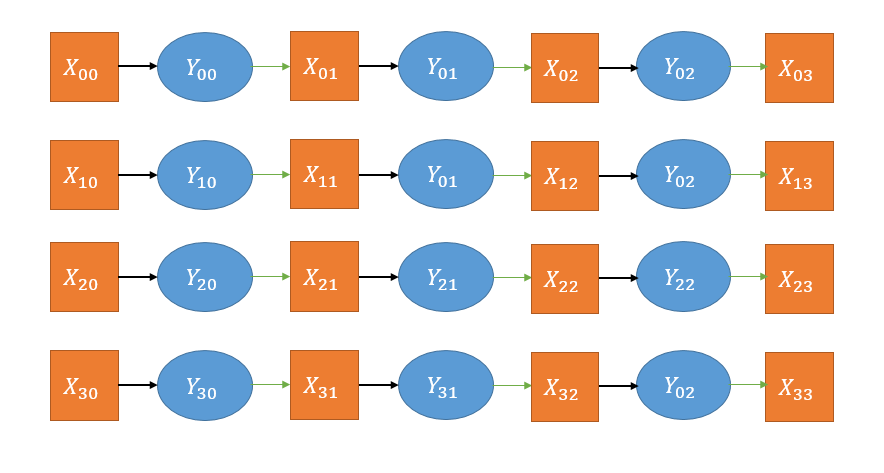
\includegraphics[width=\linewidth]{graph2}
  \caption{Pre-computation Phase}
\endminipage\hfill
\minipage{0.48\textwidth}
  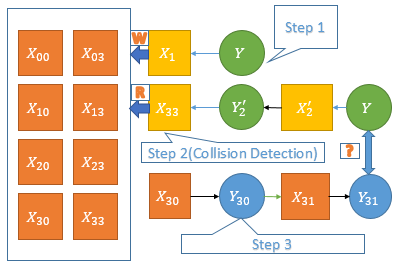
\includegraphics[width=\linewidth]{graph3}
  \caption{Online-Analysis Phase}\label{fig:awesome_image2}
\endminipage\hfill
\end{figure}

\subsubsection{Precompution.} Pre-computation takes a one way function and creates a chain of a one-way function with $t$ times. There are $m$ chains in a single table. At the end of pre-computation, starting points and ending points will be stored into files. Pre-computation is a cpu-bound problem and is identical with brute force.

In each round of a chain, it starts from $x_{i-1}$ and ends with $ x_i = R_i(H(x_{i−1})) = f_{i−1}(x_{i−1})$. $R_i$ is the reduction function and each column in the table use different reduction function, which means that $R_i(y) \neq R_j(y)$ if $i \neq j$.

\begin{exm}In \textbf{Figure 2}, there are 5 chains in a table and the length of each chain is 4. After pre-compuation, $X_{i0}$ and $X_{i3}$ will be stored into tables. Usually, endpoints should be sorted after pre-computation to reduce time of the collision detection. We will also discuss it in \textbf{Section 4}.\end{exm}

\subsubsection{Online-Anaylysis.} Online-Anaylysis can be divided into three steps.

\begin{itemize}
\item Generating the pseudo-endpoints of different length.
\item Detecting collision with the help of pre-computed tables.
\item Finally, if the collision is detected, regenerating the rest part of the chain and detecting the collision again.
\end{itemize}

\begin{exm}
\textbf{Figure 3} shows step1, step2 and step3. In step1, $X_1$, $X_{33}$ and other pseduo-endpoints will be obtained. Then, collision detection is done by comparing the pseduo-endpoints and the endpoints in the table. In this figure, $x_{33}$ is detected. Finally, regenerating the rest of chain and comparing it again.
\end{exm}

In simple terms, step 1 can be called regeneration and it will cost further more time compared with other steps. Therefore, we mainly focused on the time of regeneration.

\section{Metric Scale}
\subsection{Background}
The time-memory trade-off is a probabilistic method. Success is not guaranteed and the success rate depends on the time and memory allocated for cryptanalysis. To explain our result, we consider a basic constraint: success rate is greater than $99.0\%$. 

There are three parameters that can be adjusted in Rainbow table: the length of the chains, the number of chains per table and the number of tables produced. We assume $N, m, t, l$, respectively for size of key space, rows of a single table, columns of each table and numbers of tables. And $t_0, m_0$ are unit for time and memory. when we weigh the pros and cons of different optimization methods, we often focus on time, space and success rate. In another word, we ususally compare $T, M$ and $P_{succ}$ under different conditions.

With the increase of $m$ and $l$, the total run time and the total memory will grow linearly \cite{il1999achieving}. At the same time, the total time will be in exponent growth with the increase of $t$.

With the increase of $m$ and $t$, more identical points would be found. However, it is easy to find that when they exceed a certain limit, the increase trend will be degraded. Also, with the increase of $m$ and $t$, which means the number of different end points of a table, the probability of collision and merge will increase and more false alarms will be detected during the online-analysis phase. Success rate is determined by the number of identical points and the number of false alarms. Therefore, the success rate is difficult to be measured with different $m$, $t$ and $l$.

Therefore, it is hard to measure the pros and cons of different parameters. We will demonstrate how to solve this problem.

\subsection{Metric Scale}

\begin{defn}Relative ratio $k$, $k = \frac{mt}{N}$. Relative ratio means the amount of computation of a single table when compared with $N$. At the same time, we define the total relative ratio to be that $K = lk = l \frac{mt}{N}$.\end{defn}

For rainbow table, 
$$T = \frac{(t t_0)^2}{2} l , M = 2 (m m_0) l, k N = (m m_0) (t t_0)$$
Therefore, 
\begin{equation} 
\label{metric} TM^2 = 2 l^3 k^2 N^2
\end{equation}

The metric scale is based on (1) and we combine the time and memory together in this formula. The efficiency of different parameters is determined by $l^3 k^2$.

\begin{defn} Metric Coefficient $s$. $s = \frac{TM^2}{N^2}$. $s$ is used to represent the efficiency of different optimization methods.\end{defn}

\subsubsection{Explanations of Metric Coefficient} As we have explained, metric scale will be determined by $m$, $t$, $l$. Our proposal can use two parameters to represent it. In a nutshell, if there are two solutions for the optimization of the rainbow table, we can compare the performance by comparing the metric coefficient.

\section{Parameters Optimization}
\subsection{Best Parameters}
\begin{thm}{\cite{oechslin2003making}}
For a single rainbow table, the success rate is $$P_{sig}=1-\displaystyle\Pi_{i=1}^{t}(1-\frac{m_i}{N})$$ where $m_1 = m,~ m_{n+1} = N(1-e^{-\frac{m_n}{N}})$.  
\end{thm}

Therefore, for multiple rainbow tables, $P_{succ} = 1 - (1-P_{sig})^l$. It is easy to get $1-(1-\frac{m_t}{N})^t \leq P_{sig} \leq 1- (1-\frac{m_1}{N})^t$. Therefore, we can know $1 - e^{-\frac{m_t t}{N}} \leq P_{sig} \leq 1 - e^{-\frac{m_1 t}{N}}$.

Hellman \cite{hellman1980cryptanalytic} proposed we should choose parameters which satisfied $mt^2~=~N$ and $l~=~t$, which means $K~=~1$. Oechslin \cite{avoine2008characterization} suggested that it should be satisfied $m~=~N^{\frac{2}{3}}, t~=~N^{\frac{1}{3}}$ and $l~=~1$. However, success rate of all these methods are both $55.5\%$ in theory and practice. Therefore, large tables or multiple tables should be taken into account if we need to achieve higher success rate.

\begin{hyp} The success rate of single table is \textbf{nearly} determined by $k$. It means that the success rate of single table is almost the same, to be special, difference would be small than $1\%$, as soon as $m_1 t_1 = m_2 t_2$. We express it that $P_{sig} \approx g(k)$.\end{hyp}

We conduct some experiments of different parameters and show them in \textbf{Table 1} to explain the Hypothesis. This figure clearly shows that the difference of success rate with different $k$ is very small. With the increase of the number of tables, the difference of success rate will become smaller and smaller.

\begin{table}
  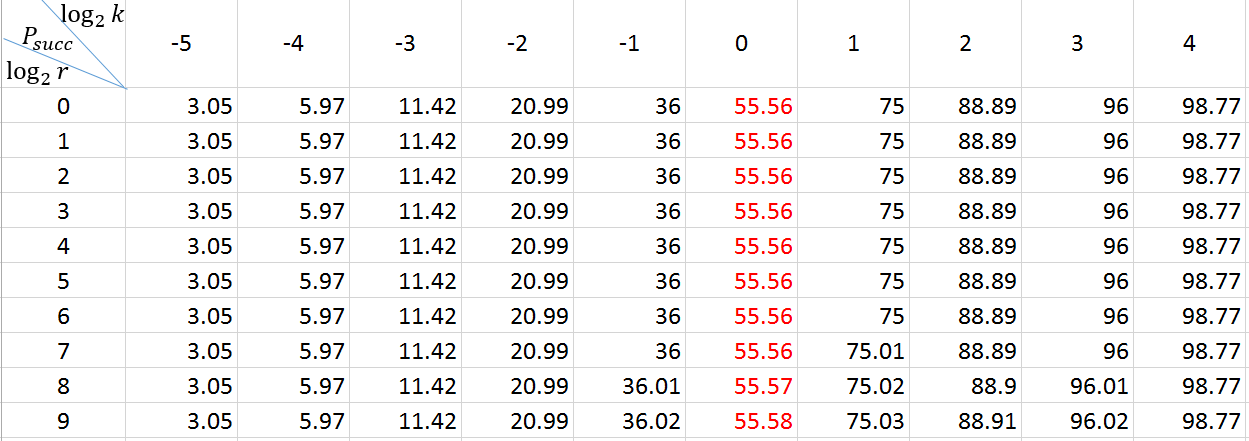
\includegraphics[width=\linewidth]{table1}
  \caption{$N = 2^{37}$. $k = \frac{m \times t}{N}$ and $r^2 = \frac{m}{t}$.  Each column represents the trend of change with the special parameters. Same success rate (approx) can be observed in the same column}
\end{table}

Based on this assumption, we can draw \textbf{Figure 4}. This figure shows how to obtain the corresponding success rate from k and  how to obtain the k by the corresponding success rate.

\begin{figure}[!htb]
\minipage{0.48\textwidth}
  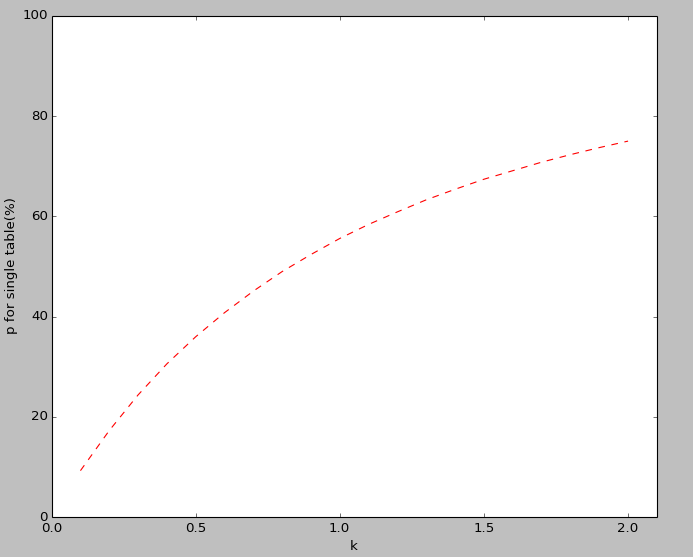
\includegraphics[width=\linewidth]{graph4}
  \caption{Relationship between $k$ and $P_{sig}$. It can be used to obtain any k according different success rate of single table.}
\endminipage\hfill
\minipage{0.48\textwidth}
  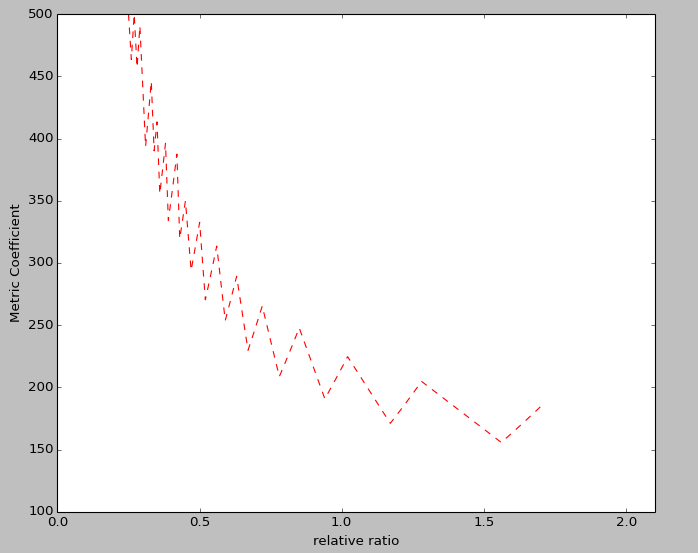
\includegraphics[width=\linewidth]{graph5}
  \caption{Relationship between $k$ and $l^3 k^2$. From it, we can know that $k = 1.56$ is the best choice.}
\endminipage\hfill
\end{figure}

We have known $$P_{succ} = 1- (1 - P_{sig})^l~,~P_{sig}~=~g(k)$$

Therefore, $$l = \ceil[\big]{log_{g(k)} (1-P_{succ})} $$ $$TM^2 = 2(\ceil[\big]{(log_{g(k))} (1-P_{succ})})^3 k^2 N^2 = R(g(k), P_{succ}) N^2$$ 
\begin{equation} 
\label{metric} s = 2(\ceil[\big]{(log_{g(k))} (1-P_{succ})})^3
\end{equation}

\begin{table}
  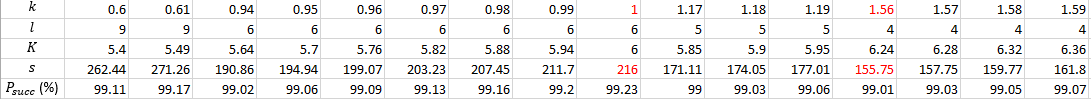
\includegraphics[width=\linewidth]{table2}
  \caption{Relationship between $k$ and $s$. From it, we can conclude  $k = 1.56$ can save about $\frac{216−155}{216} \approx 28.2\%$.}
\end{table}

(2) shows that $s$ is determined by $k$ and $P_{succ}$ and we have stated that $P_{succ} > 99.0\%$ in previous section. Therefore, $s$ is determined by $k$ in the case of fixed success rate. We shows our experiment result in \textbf{Figure 5} and \textbf{table 2} with different $k$. It demonstrates that $k = 1.56$ and $l = 4$ is the perferable than $k = 1, l = 6$ when $N = 2^{37}$. The parameters we choose can achieve $28\%$ improvement in metric coefficient. The improvment for time and space will be disccussed in 6.3.

\begin{algorithm*}[!ht]
\DontPrintSemicolon
\KwIn{the size of key space, which means $N$. The lower bound of success rate, which means $P_{succ}$}
\KwOut{$k$}
\Begin{
	$arr = []$\;
	\For{$k$ in $[0.1~\to~2.0]$}
    {
      Getting $g(k)$\;
      Computing $(\ceil[\big]{(log_{g(k))} (1-P_{succ})})$. Marking it as $l$\;
      Compute $l^3 k^2$ and append it to \textbf{arr}\;
    }
    Find the smallest element in \textbf{arr} and find the corresponding parameter $k$.\;
    return $k$\;
}
\caption{General Method to get the best $k$.}
\end{algorithm*}

\subsection{General Method}
\subsubsection{Algorithm 1}: In previous subsection, we conclude that $s$ is  determined by different $s$ and $P_{succ}$ and we present the pseudocode in Algorithm 1.

\subsubsection{Algorithm 2}: Hypothesis 1 states that $P_{sig} \approx g(k)$ and it gives us a general method to choose best parameters with given success rate. However, we give out Hypothesis 1 without any proof and we should notice that no matter whether it is right or wrong for different $N$, it will also give us a choice to find better parameters compared with traditional ones. And we present another general algorithm in Algorithm 2.


\begin{algorithm*}[!ht]
\DontPrintSemicolon
\KwIn{the size of key space, which means $N$. The lower bound of success rate, which means $P_{succ}$}
\KwOut{$k$}
\Begin{
	$arr = []$\;
	\For{$k$ in $[0.1~\to~2.0]$}
    {
      Getting $g(k), m = (kN)^{\frac{2}{3}}, t = (kN)^{\frac{1}{3}}$\;
      Computing $(\ceil[\big]{(log_{g(k))} (1-P_{succ})})$. Marking it as $l$\;
      Compute $l^3 k^2$ and append it to \textbf{arr}\;
    }
    Find the smallest element in \textbf{arr} and find the corresponding parameter $k$.\;
    return $k$\;
}
\caption{General Method to get the best $k$ without \textbf{Hypothesis 1}}
\end{algorithm*}

\subsection{Discussion In-Depth}

$l$ should be an integer and it can produce a small difference of success rate and we hope to generate the exactly the same success rate and these difference have slight impact on performance. We will give an example to produce $99.0\%$  of the success rate.

$$P(k = 1) = 55.5\%, 1 - (1 - P(k = 1))^6 = 0.9916$$
And, 
$$1 - (1 - 0.5)(1 - P(k = 1))^5 = 0.9907$$
Therefore, we can compute five tables as same as origin method and we only need to generate the rest table which the success rate for this table is $50\%$, which means $k = 0.85$. This tip can save about $2.5\%$ time for pre-computation and save about $4\%$ cryptanalyis time. So, it won't affect our \textbf{metric scale}.

\section{Improved Table Structure}

We have stated that Rainbow Table suffers an obvious benefit from the size of single table. However, the main limitation of the original rainbow scheme is the fact that the time of regenerating will be in exponent growth with $t$\cite{oechslin2003making}.  
$$1 + 2 + 3 + ... + t \approx \frac{t^2}{2}$$
At the same time, classic table will be in linearly growth\cite{hellman1980cryptanalytic} with the length of chain.
$$1 + 1 + 1 + ... + 1 \approx t$$.
Therefore, we hope to be able to combine the two types of table together and propose a new table structure.
\subsection{Our Structure}
Our structure utilizes the same reduction function in the first half and uses successive reduction functions in the rest of the chain. \textbf{Figure 6} and \textbf{Figure 7} shows the difference between origin rainbow table and our improved table structure.

\begin{figure}[!htb]
\minipage{0.48\textwidth}
  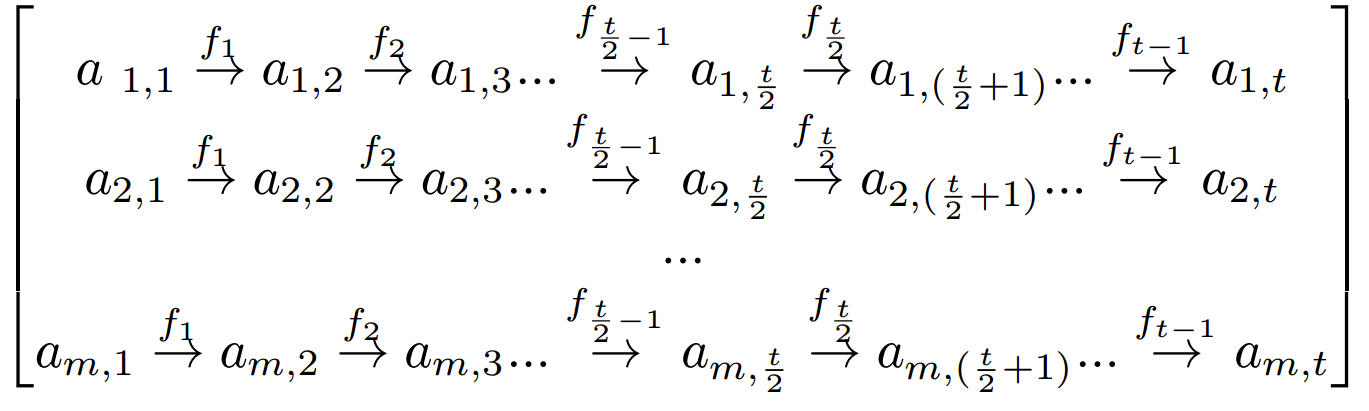
\includegraphics[width=\linewidth]{graph6}
  \caption{Rainbow Table. Using different reduction functions in each column of the matrix.}
\endminipage\hfill
\minipage{0.48\textwidth}
  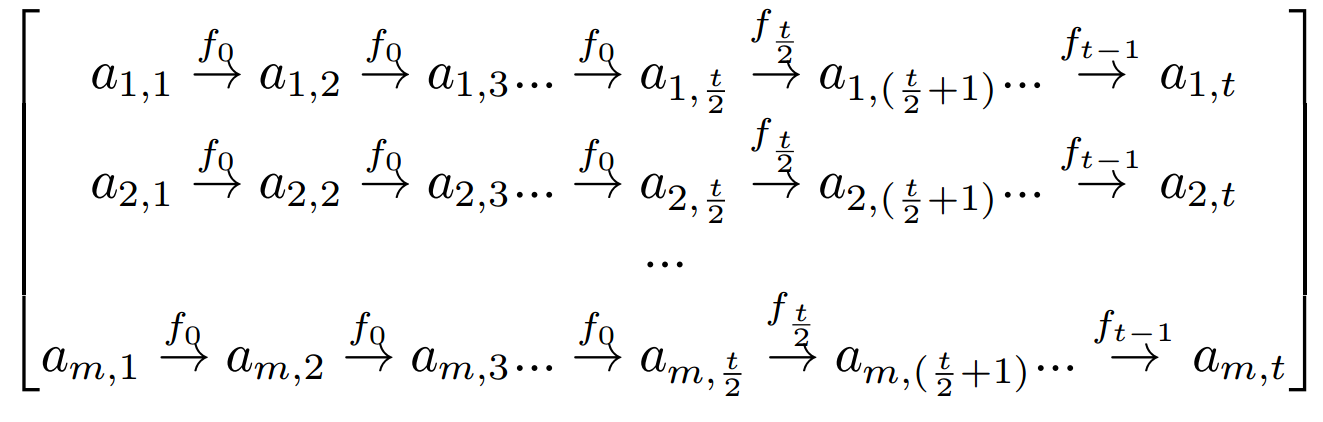
\includegraphics[width=\linewidth]{graph7}
  \caption{Improved Structure. Using both the same reduction function and different reduction functions.}
\endminipage\hfill
\end{figure}

In theory, the regeneration of new table structure will cost 
$$\frac{t}{2} + \frac{t}{2}∗\frac{t}{2} + (1 + 2 + ...+ \frac{t}{2}) \approx \frac{3}{8} t^2$$
Therefore, for new table, we can get 
$$T = (\frac{t}{2} + \frac{3t^2}{8})t_0 l = \frac{3}{8} (tt_0)^2 , M = 2(mm_0)l, k N = (mm_0) t$$ 
So, we can know 
$$TM^2 = \frac{3}{2}(l^3 k^2 N^2) N^2$$

Therefore, the run-time of regeneration phase can be decreased by $25\%$.

Based on previous result, we choose several parameters for rainbow table and verify the efficiency of improved table structure. The results are given in \textbf{Figure 10}:

\begin{table}
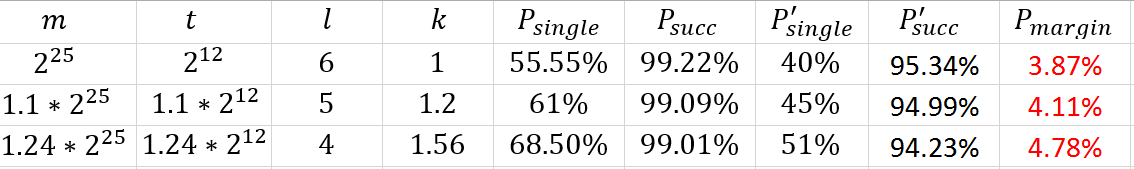
\includegraphics[width=\linewidth]{table3}
\caption{Performance of Improved Structure. $P_{single}^{'}$ means the success rate of the improved single table and $P_{succ}^{'}$ means the success rate of the improved table. $P_{margin} = P_{succ} - P_{succ}^{'}$.}
\end{table}
We have shown that improved structure can achieve $25\%$ improvement in time and the success rate would decrease by no more than $5\%$. We can note that with the increse of relative ratio, the margin also increased. That means that our improved table structure is preferable when there are many subtables. 

There is another variant of this table, which was shown in \textbf{Figure 11}. It will costs 
$$T = (((\frac{t}{2}) + (\frac{t}{2}+1) + ... + t) + \frac{t}{2}) l\approx \frac{t^2}{2} l$$ 
So it can't promote any optimization.

\begin{figure}
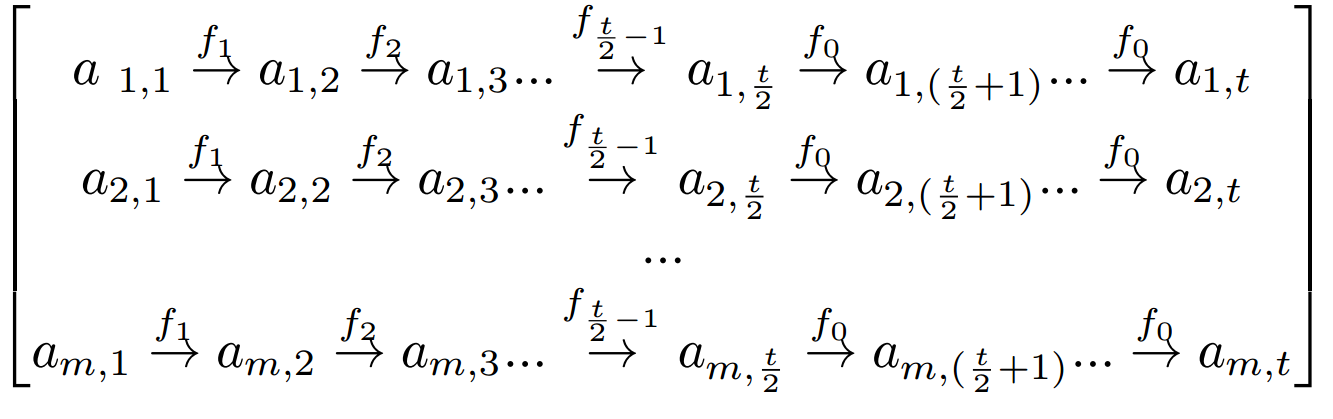
\includegraphics[width=\linewidth]{graph8}
\caption{Another Improved Structure. With different order of reduction functions.}
\end{figure}

\subsection{Another Benefit of Our Structure}

There are two benefits of Hellman's work. The first one has been introduced in previous sub-section and the second benefit is that classic table can save large of memory compared with Rainbow Table. We will discuss it in detail in this subsection. In the end of this subsection, we will conclude that our improved table structure can also benefit from it.

The memory size refers to the total size of starting points and ending points. There are many technologies for memory optimization. The most obvious method is that we can reduce the number of pairs of points. Another method is trying to save the storage requriement of each pair. Each pair of starting point and ending point can surely be stored in $2 log_2 N$ bits. There are two methods to save the space of each pair.

Firstly, for starting points, we can choose consecutive points instead of random points\cite{barkan2006rigorous}. In that way, $log_2 m$ bits, instead of $log_2 N$, is required for each starting point.

Secondly, during the online phase, the calculated $X^{'}$ is compared with the sorted ending points in the table. The best method is to use index table. Index table is a degenerated form of hash table. In a nutshell, the ending points computed in pre-computation phase should be sorted in advance and each point will be divided into two parts. The length of first part is $\eta$ and the length of rest is $log N  - \eta$. As there are $\frac{m}{2^\eta}$ points share the same prefix of length $\eta$ in the set of end points, the length of each end point can be calculated as $log_2 N - \eta + \frac{\eta 2^\eta}{m}$. It is easy to get that $\eta = log_2 m - 1$ is preferable. 

When we have used the two methods mentioned above, $m_0^{'} = log_2 m + log N - \eta + \frac{\eta 2^\eta}{m}$ instead of $m_0 = 2 log_2 N$. We should notice that $log_2 m > \eta$.

The next idea, which is shown in Figure 10, for staring points is that we can store $log_2 m$ instead of $m log_2 m$\cite{spitz2007time} for starting points. The side effect of this solution is a table which can no longer be sorted by the ending points which increase the search times during the online phase. In collision detection phase, it will costs $t log_2(m)$ for sorted ending points. Therefore, if the endings points aren't sorted in advanced, it will cost $m log_2(t)$. 

\begin{figure}[!htb]
\minipage{0.48\textwidth}
  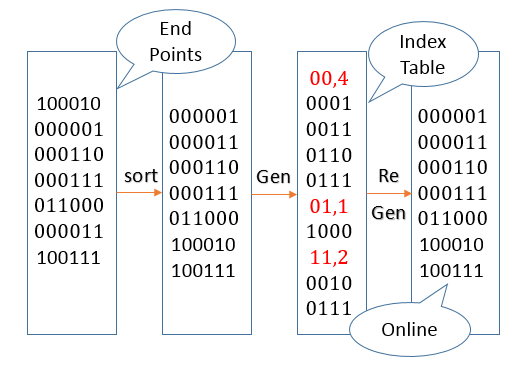
\includegraphics[width=\linewidth]{graph9}
  \caption{Index Table technique. There are three steps in it. Firstly, sorting the ending points. Then use index table to save space. Finally, during cryptanalysis, transforming the index table to sorted table.}
\endminipage\hfill
\minipage{0.48\textwidth}
  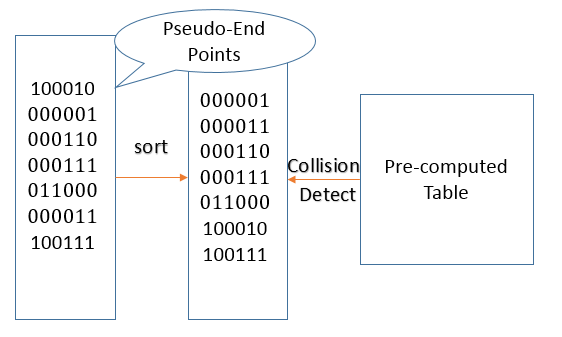
\includegraphics[width=\linewidth]{graph10}
  \caption{The Next Idea We Suggest. In phase of collision detection, sorting the pseduo-end points firstly. Then, using the pre-computed table, which won't be sorted in advance, to detect collision.}
\endminipage\hfill
\end{figure}

Thus, if we take $m~=~t$, the saving of starting points won't give any burden compared with previous optimization. We have known that $m = N^{\frac{1}{3}}, t = N^{\frac{1}{3}}, l = N^{\frac{1}{3}}$.

If we take the method into consideration, $m_0^{''} = \frac{log_2 m}{m} + log_2 N \approx log_2 N$. In a simple way, $m_0^{'} - m_0^{''} = log_2 m - \eta + \eta \frac{2^\eta}{m}$. It is easy to notice that $m_0^{'} - m_0^{''} > 0$. Therefore, the optimization technology can be utilized to save storage and it is the another benefit we have mentioned above.

We should notice that $m = t$ will leads that $T = \frac{(tt_0)^2}{2}l = \frac{kN t_0^2}{2}$ in rainbow table. In our improved table structure, we have calculated that regeneration will cost $\frac{3}{8} t^2$ instead of $\frac{t^2}{2}$. Therefore, if $m~=~t$, it is better than the origin rainbow scheme.

\section{Experimental Results}
\subsection{Attack Platform}
We have chosen cracking of NTLM as an example because it has a real significance in our life.

In Windows, NT LAN Manager (NTLM) \cite{malhotra2013review} is a suite of Microsoft security protocols that provides authentication, integrity, and confidentiality to users and NTLM is based on NT-Hash function. NT-hash function is the default hash function used by Windows 7 and 8.

NT-Hash uses MD4 as the internal hash-function and there are two steps in it,

1. Change the source password into Unicode representation using little-endian.

2. Using MD4 to generate the target hashed-password. The length of hashed-password is 128 bits.

In our experiments, we choose 6 words and each words can choose from $a - z, A - Z, 0 - 9$ and ten common special characters. The total space of keys is $7^{26} \approx 2^{37}$. We need to notice that our experiments can be applied to any hash-based function, such as DES and FEAL-32 \cite{kusuda1996optimization}.

\subsection{Experimental Results}
Based on \textbf{Parameter Selection} and \textbf{Improved Table Structure}. we have chosen the parameters for origin rainbow table to be $m_0 = 2^{25}, t_0 = 2^{12}, l_0 = 6, \eta = 24$ and the parameters for improved table to be $m_1 = 2^{25}*\sqrt{1.56}, t_1 = 2^{12}*\sqrt{1.56}, l_1 = 4, \eta = 24$. We have generated 1000 random password and try to crack them in our PC (Thinkpad T430U, Intel i5-3317 and 4G RAM). The result are given in the \textbf{Table 4},

\begin{table}
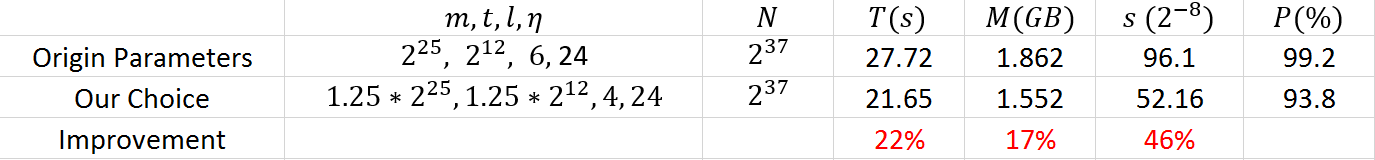
\includegraphics[width=\linewidth]{table4}
\caption{Experiment 1. The combination of two methods.}
\end{table}

This experiments shows that it can achieve the time can decrease by $22\%$ time and the space can decrease by $17\%$ with the cost of $5.4\%$ in success rate. In summary, 1 - $\frac{T_1 M_1^2}{T_0 M_0^2} \approx 46\%$.

In \textbf{5.2}, we state that our table suffered from another benefit transformed by the Hellman's Table. We choose $m_2 = 2^{19}*\sqrt{1.56}, t_2 = 2^{18}*\sqrt{1.56}, l_1 = 4$ and use the optimization mentioned in 5.2. The result are shown in the \textbf{Table 5}.

\begin{table}
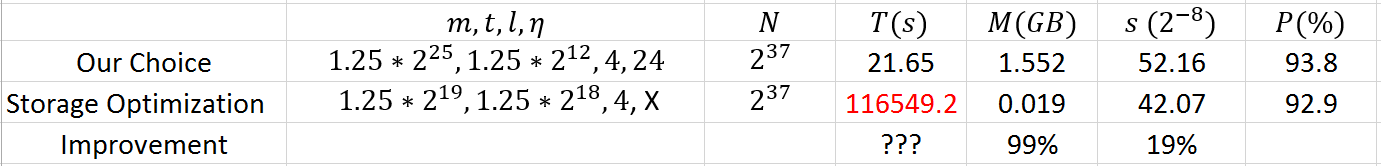
\includegraphics[width=\linewidth]{table5}
\caption{Experiment 2. Optimization mentioned in 5.2}
\end{table}

What we can see from this table is that $1 - \frac{T_2 M_2^2}{T_0 M_0^2} \approx 19\%$ with the cost of $1\%$ in success rate.

\subsection{Increasing the Gain Even Further}

In above result, we find out that $s$ will decrease by $46\%$. At some point, we need to know specifically what is bound it can bring from time or memory individually.

For origin Rainbow Table, 
$$T_0 = 6t^2, M_0 = 6m$$
For $k = 1.56$,
$$T_1^{'} = \frac{1}{2} a^2 T_0, M_1^{'} = \frac{1.56*4}{6 a} M_0 = \frac{1.04}{a} M$$

Therefore, we get $m_3 = \frac{1.56}{1.04} N^{\frac{2}{3}}, t_3 = 1.04 N^{\frac{1}{3}}$ and $m_4 = \frac{1.56}{0.5} N^{\frac{2}{3}} = 3.12 N^{\frac{2}{3}}, t_4 = 0.5 N^{\frac{1}{3}}$. $m_3$ and $m_4$ respectively lead same memory and time compared with the classic rainbow schema. 

\begin{table}
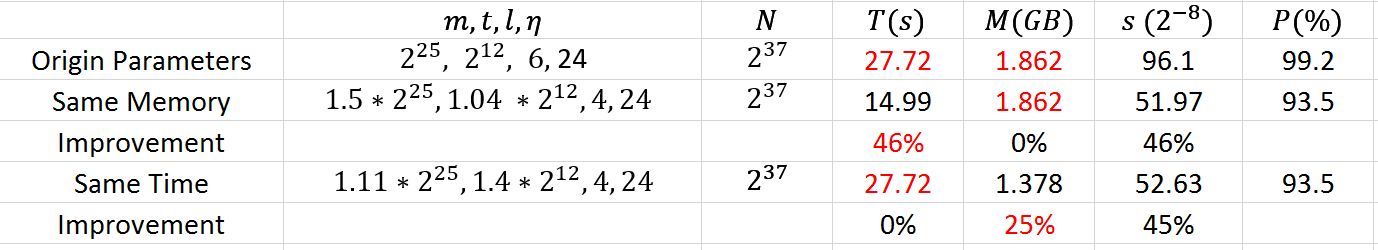
\includegraphics[width=\linewidth]{table6}
\caption{Experiment 3. This experiment is used to explore the upper bound of time and memory.}
\end{table}

In \textbf{Table 6}, we compare the average cryptanalysis time and the average cryptanalysis memory with $m_3, t_3$ and $m_4, t_4$. From the experimental results, we see that the time can be reduced by up to $46\%$ and the space can be reduced by up to $25\%$.

\section{Conclusion}

In this paper, we introduce a metric scale to determine the benefits of different parameters and we also introduce some ways to reduce the cost of time and memory during cryptanasis in Rainbow Table. 

The first optimization suffers benefit from the scale. Based on the new scale, we achieve several improvements for Rainbow Table and present a pseudo-code for general $N$. In practical, the time can decrease by $28\%$ and the space will decrease by $15\%$ compared with previous work.

The second optimization suffers benefit from both the Hellman's table and Rainbow Table. In the second part of this paper, we find out that Rainbow Table suffere some leakages compared with classic table. Therefore, we try to introduce an improved table structure and show the benefits of our proposal. It can benefit both from linear computation and storage optimization. Our analysis yields $25\%$ improvements of time with the cost of $5\%$ of success rate. 

Finally, we conducte our experiments in an attack platform and our experiment has demonstrated that the time-memory trade-off allows anybody owning a modern personal computer to break NTLM problems. Our experiments also introduce how to solve optimization problem for time or memory. Through our experiments, we shows that memory can be transfered to time and time can be transfered to memory in the different direction.

We hope that our paper can assist you to find the best parameters in different atmosphere and can open your mind to find other table structure.

\bibliographystyle{abbrv}
\bibliography{paperbib} 
\end{document}